\documentclass[12pt, letterpaper]{../assignment}
\usepackage{graphicx}
\usepackage{courier}
\usepackage{minted}
\usepackage{amsmath}
\usepackage{polynom}
\usepackage{commath}
\usepackage{amssymb}
\usepackage{amsfonts} 
\usepackage{enumitem}
\usepackage{color}
\usepackage{cancel}
\usepackage{enumitem}
\usepackage{graphicx}
\usepackage{multirow}
\usepackage{float}
\usepackage{bm}
\usepackage{tikz}
\usetikzlibrary{shapes,arrows}
\usepackage{booktabs}
\usetikzlibrary{patterns}

% Define Theme Colors
\definecolor{light-gray}{rgb}{0.2,0.2,0.2}
\definecolor{header-blue}{rgb}{0,0,0.7}
% \definecolor{header-blue}{rgb}{0.5137,0.8353,0.9176}
\definecolor{header-blue}{rgb}{0,0.8,0.95}
%\definecolor{dark-gray}{rgb}{0.1,0.1,0.1}
\definecolor{dark-gray}{rgb}{0.07,0.07,0.07}
\pagecolor{dark-gray}
\color{white}

\usemintedstyle{monokai}
\oddsidemargin = 0pt
\exercisesheet{Module 14}{Final Exam}
\student{Austin Barrilleaux}
\university{\color{header-blue}Johns Hopkins University}
\school{\color{header-blue}Whiting School of Engineering}
\courselabel{EN 535.612}
\semester{Fall 2024}
\usepackage[backend=bibtex,style=numeric,sorting=none]{biblatex}
\bibliography{reference}

\definecolor{light-gray}{rgb}{0.2,0.2,0.2}
\setminted{bgcolor=light-gray,frame=lines,rulecolor=white}
\setlength{\parindent}{0pt}

\makeatletter
\patchcmd{\minted@colorbg}{\noindent}{\medskip\noindent}{}{}
\apptocmd{\endminted@colorbg}{\par\medskip}{}{}
\makeatother

\begin{document}

\subsection*{Problem 1}
\subsubsection*{The wheelbarrow is pushed in the horizontal plane by forces $\bm{F_1 = [F_{1_x}, F_{1_y}]^T}$ and $\bm{F_2 = [F_{2_x}, F_{2_y}]^T}$ acting at the ends of the handles.
See Fig. 1 for the graphical explanation of the system.
The chassis has mass m, with its center of mass situated at point $\bm{G}$ on the centerline.
The centroidal moment of inertia of the chassis about a vertical axis (the $\bm{Z}$-axis) is $\bm{I}$.
The wheel, which may be approximated as a thin disk (hence inertia can be ignored),
rolls without slipping.
The position of G is denoted as $\bm{(x, y)}$ and the steering angle is denoted as $\bm{\theta}$.}


\begin{figure}[H]
  \centering
  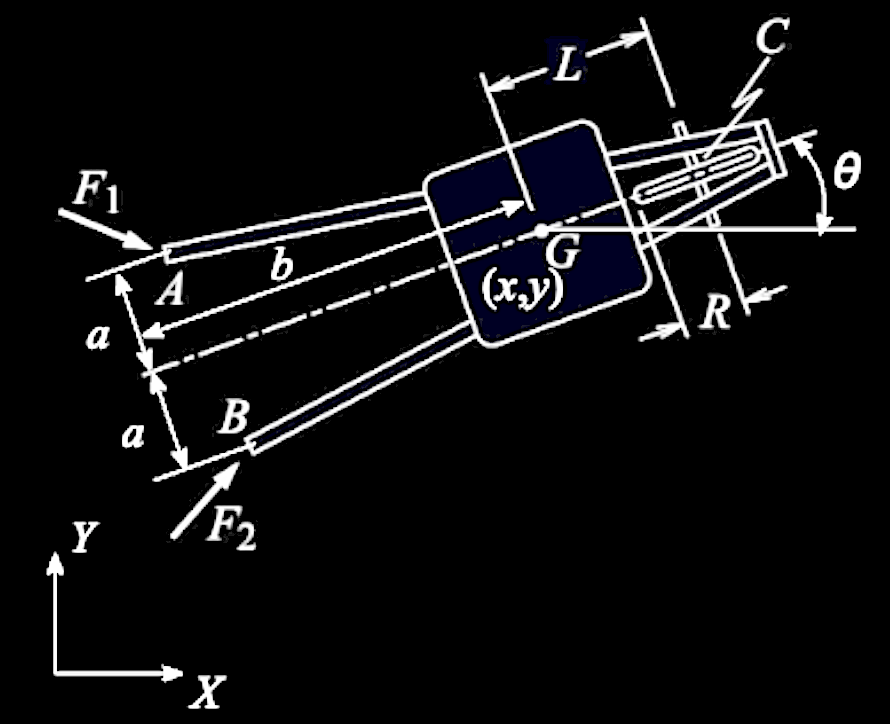
\includegraphics[scale=0.5,frame]{images/Problem_1.png}
%  \caption{Problem 2: 5 rev/s is applied to part (b).}
\end{figure}

Convenient generalized coordinates for the wheelbarrow are the absolute position coordinates of point G, 
$q_1 = x$, $q_2 = y$, and the angle $q_3= \theta$ locating the x-axis relative to a fixed XYZ reference frame.
\\\\

The position of the chassis is:

$$ r_G = \left<\begin{array}{c}
x\\
y\\
0
\end{array}\right> $$

Its derivative yields:

$$ v_G = \left<\begin{array}{c}
\dot{x}\\
\dot{y}\\
0
\end{array}\right> $$

The position of the wheel is:

$$ r_C = \left<\begin{array}{c}
x+L\,\cos \left(\theta \right)\\
y+L\,\sin \left(\theta \right)\\
0
\end{array}\right> $$

Its derivative yields:

$$ v_C = \left<\begin{array}{c}
\dot{x}-L\,\sin \left(\theta \right)\,\dot{\theta} \\
\dot{y}+L\,\cos \left(\theta \right)\,\dot{\theta} \\
0
\end{array}\right> $$


\subsubsection*{(a) Derive the velocity constraint form.}

The velocity constraint exists due to the no-slip condition where the wheel contacts the ground,
directly below the cm of the wheel.
Due to this constraint, the velocity in the $j$ direction must be zero.
This is described as:

\begin{equation*}
  \begin{aligned}
    v_C \cdot j &= 0 \\
      &= \left<\begin{array}{c}\dot{x}-L\,\sin \left(\theta \right)\,\dot{\theta} \\\dot{y}+L\,\cos \left(\theta \right)\,\dot{\theta} \\0\end{array}\right>
         \cdot \left<\begin{array}{r} -\sin\left(\theta \right)\\ \cos\left(\theta \right)\\ 0 \end{array}\right> \\
      &= -\sin \left(\theta \right)\,\dot{x} +\cos \left(\theta \right)\,\dot{y}+ L\,\dot{\theta}=0
  \end{aligned}
\end{equation*}

The velocity constraint is:

\begin{answer}
$$-\sin \left(\theta \right)\,\dot{x} +\cos \left(\theta \right)\,\dot{y}+ L\,\dot{\theta}=0$$
\end{answer}

Putting this in the form of the constraint equation:

$$ \sum_{j=1}^N a_{ij} \dot{q}_j + b_i =
a_{11} \dot{q}_1 + a_{12} \dot{q}_2 + a_{13} \dot{q}_3 + b_1 = 0  $$

We see that:

\begin{answer}
\begin{equation*}
    \begin{aligned}
        a_{11} &= -\sin \left(\theta \right) \\
        a_{12} &= \cos \left(\theta \right) \\
        a_{13} &= L
    \end{aligned}
\end{equation*}
\end{answer}

\subsubsection*{(b) Derive the Lagrange equations of motion.
Express equations with given parameters in the problem.}

Given that the inertia of the wheel can be ignored,
and as a result there is no rotational or translational energy component for the wheel,
the kinetic energy of the system is described as:

$$ T = \frac{1}{2} m \left(v_G \cdot v_G \right) +
       \frac{1}{2} I \dot{\theta}^2 $$

Where potential energy, $V = 0$, so $L = T$.
\\\\
This evaluates to::

$$ L = \frac{1}{2}\textrm{I}\,{{\dot{\theta} }}^2 +\frac{1}{2}m\,{{\dot{x}}}^2 +\frac{1}{2}m\,{{\dot{y}}}^2 $$

Solving for the generalized forces, the virtual work for the system is:

\begin{equation*}
  \begin{aligned}
    \delta W &= \sum_{j=1}^N Q_j \delta q_j \\
             &= F_1 \cdot \delta r + F_2 \cdot \delta r + M \cdot \delta \theta \\
             &= \left( F_1 + F_2 \right) \cdot \left< \begin{array}{ccc} \delta x \\ \delta y \end{array} \right> + M \cdot \delta \theta \\
             &= \left( F_1 + F_2 \right) \cdot I\ \delta x + \left( F_1 + F_2 \right) \cdot J\ \delta y + \left(r_{A/G} \times F_1 + r_{B/G} \times F_2\right) \delta \theta
  \end{aligned}
\end{equation*}

Therefore, the generalized forces are:

\begin{equation*}
  \begin{aligned}
      Q_x &= \left( F_1 + F_2 \right) \cdot I\\
      Q_y &= \left( F_1 + F_2 \right) \cdot J\\
      Q_\theta &= \left(r_{A/G} \times F_1 + r_{B/G} \times F_2\right)
  \end{aligned}
\end{equation*}

Because the forces were not provided as vectors, I cannot describe the terms more precisely.
\\\\
Solving for the equations of motion along the generalized coordinate, $x$:

$$ \frac{d}{d t} \frac{\partial L}{\partial \dot{x}} - \frac{\partial L}{\partial x} = 
Q_{x} + a_{11} \lambda_1 $$

The component parts of this equation are:


$$ \frac{\partial L}{\partial x} = 0 $$

$$ \frac{\partial L}{\partial \dot{x}}  =
m\,\dot{x} $$

$$ \frac{d}{d t} \frac{\partial L}{\partial \dot{x}} =
 m\,\ddot{x} $$

 This results in the equation of motion:
 
 $$ m\,\ddot{x} =
 \left( F_1 + F_2 \right) \cdot I -\sin \left(\theta \right) \lambda_1 $$

 Solving for the equations of motion along the generalized coordinate, $y$:

 $$ \frac{d}{d t} \frac{\partial L}{\partial \dot{y}} - \frac{\partial L}{\partial y} = 
 Q_{y} + a_{12} \lambda_1 $$
 
 The component parts of this equation are:
 
 
 $$ \frac{\partial L}{\partial y} = 0 $$
 
 $$ \frac{\partial L}{\partial \dot{y}}  =
 m\,\dot{y} $$
 
 $$ \frac{d}{d t} \frac{\partial L}{\partial \dot{y}} =
m\,\ddot{y} $$
 
This results in the equation of motion:
  
$$ m\,\ddot{y} =
\left( F_1 + F_2 \right) \cdot J +\cos \left(\theta \right) \lambda_1 $$

Solving for the equations of motion along the generalized coordinate, $\theta$:

$$ \frac{d}{d t} \frac{\partial L}{\partial \dot{\theta}} - \frac{\partial L}{\partial \theta} = 
Q_{\theta} + a_{13} \lambda_1 $$

The component parts of this equation are:


$$ \frac{\partial L}{\partial \theta} = 0 $$

$$ \frac{\partial L}{\partial \dot{\theta}}  =
\textrm{I}\,\dot{\theta}  $$

$$ \frac{d}{d t} \frac{\partial L}{\partial \dot{\theta}} =
\textrm{I}\,\ddot{\theta}  $$

 This results in the equation of motion:
 
 $$ \textrm{I}\,\ddot{\theta}  =
 r_{A/G} \times F_1 + r_{B/G} \times F_2 + L \lambda_1 $$

The Lagrange equations of motion are:

\begin{answer}
  \begin{equation*}
    \begin{aligned}
      m\,\ddot{x} &= \left( F_1 + F_2 \right) \cdot I -\sin \left(\theta \right) \lambda_1 \\
      m\,\ddot{y} &= \left( F_1 + F_2 \right) \cdot J +\cos \left(\theta \right) \lambda_1 \\
      \textrm{I}\,\ddot{\theta} &= r_{A/C} \times F_1 + r_{B/C} \times F_2 + L \lambda_1
    \end{aligned}
  \end{equation*}
\end{answer}

The following MATLAB script was used to solve this problem:

% \color{white}
\hspace*{6em}\inputminted[frame=leftline,fontsize=\scriptsize,lastline=50]{matlab}
{./matlab/Problem_1.m}
% \color{black} 

\subsection*{Problem 2}

\begin{figure}[H]
    \centering
    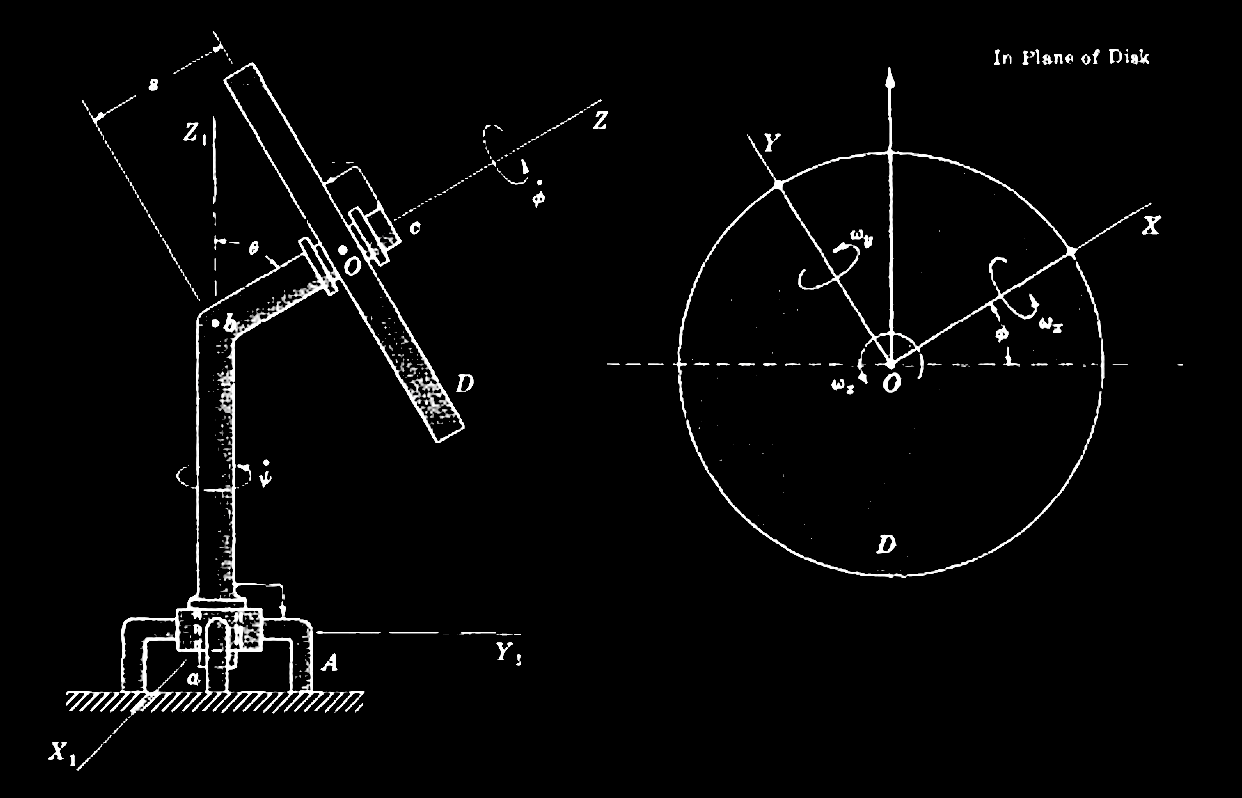
\includegraphics[scale=0.6,frame]{images/Problem_2.png}
  %  \caption{Problem 2: 5 rev/s is applied to part (b).}
\end{figure}

\subsubsection*{Consider the system in Fig. 2. Frame $\bm{\{X_1 Y_1 Z_1\}}$ is the spatially fixed frame,
and $\bm{\{XYZ\}}$ is the body-fixed frame attached to the disk (the origin $\bm{O}$ is at the center of mass of the disk).
A is at rest.
The origin $\bm{O}$ of the body-fixed frame is at the center of mass of the disk.
The bar $\bm{ab}$ (hence the elbow) is rotating about the $\bm{Z_1}$-axis and its rotation angle is denoted as $\bm{\psi}$.
The length of the bar ab is $\bm{L}$.
Angle $\bm{\theta}$ is constant, as you can see in the figure.
Finally the disk is rotating about the $\bm{Z}$-axis and its rotation angle is denoted as $\bm{\phi}$.
Mass of the disk is $\bm{M}$, and the moment of inertia matrix (body quantity) is
$$\bm{ I_b = \textbf{diag}[I_x, I_x, I_z ]}$$
We only consider the motion of the disk.
In other words, we ignore the mass and inertia of the elbow.
For this problem, use the approach in Module 13.}

\subsubsection*{(a) Compute the kinetic energy of the system
(Hint: use the $\bm{ZXZ}$ Euler angles to describe the orientation of the disk (i.e., $\bm{\{XYZ\}}$) relative to $\bm{\{X_1 Y_1 Z_1\}}$).}

Using the $ZXZ$ Euler angles to represent the orientation of the disk:

\begin{equation*}
  \begin{aligned}
    R_{ZXZ} &= R_{Z}(\psi) R_{X}(\theta) R_{Z}(\phi) \\
    &= \left[\begin{array}{ccc} \cos\left(\psi \right) & -\sin\left(\psi \right) & 0\\ \sin\left(\psi \right) & \cos\left(\psi \right) & 0\\ 0 & 0 & 1 \end{array}\right]
    \left[\begin{array}{ccc} 1 & 0 & 0\\ 0 & \cos\left(\theta \right) & -\sin\left(\theta \right)\\ 0 & \sin\left(\theta \right) & \cos\left(\theta \right) \end{array}\right]
    \left[\begin{array}{ccc} \cos\left(\phi \right) & -\sin\left(\phi \right) & 0\\ \sin\left(\phi \right) & \cos\left(\phi \right) & 0\\ 0 & 0 & 1 \end{array}\right]\\
    &= \footnotesize{\left[\begin{array}{ccc}
            \cos \left(\phi \right)\,\cos \left(\psi \right)-\cos \left(\theta \right)\,\sin \left(\phi \right)\,\sin \left(\psi \right) & -\cos \left(\psi \right)\,\sin \left(\phi \right)-\cos \left(\phi \right)\,\cos \left(\theta \right)\,\sin \left(\psi \right) & \sin \left(\psi \right)\,\sin \left(\theta \right)\\
            \cos \left(\phi \right)\,\sin \left(\psi \right)+\cos \left(\psi \right)\,\cos \left(\theta \right)\,\sin \left(\phi \right) & \cos \left(\phi \right)\,\cos \left(\psi \right)\,\cos \left(\theta \right)-\sin \left(\phi \right)\,\sin \left(\psi \right) & -\cos \left(\psi \right)\,\sin \left(\theta \right)\\
            \sin \left(\phi \right)\,\sin \left(\theta \right) & \cos \left(\phi \right)\,\sin \left(\theta \right) & \cos \left(\theta \right)
            \end{array}\right]}
  \end{aligned}
\end{equation*}


We can compute the body angular velocity as:

$$ \omega_b = \textbf{vect}\left(  R^T \dot{R} \right) =
\left<\begin{array}{c} \sin\left(\phi \right)\,\sin\left(\theta \right)\,\dot{\psi} \\ \cos\left(\phi \right)\,\sin\left(\theta \right)\,\dot{\psi} \\ \dot{\phi} +\cos\left(\theta \right)\,\dot{\psi}  \end{array}\right>$$

The location of the center of the disk is:

$$ r = \left<\begin{array}{c}
L+s\,\sin \left(\psi \right)\,\sin \left(\theta \right)\\
-s\,\cos \left(\psi \right)\,\sin \left(\theta \right)\\
s\,\cos \left(\theta \right)
\end{array}\right> $$

Taking its derivative, the velocity of the center of mass of the disk is:

$$ v = \left<\begin{array}{c}
s\,\cos \left(\psi \right)\,\sin \left(\theta \right)\,\dot{\psi} \\
s\,\sin \left(\psi \right)\,\sin \left(\theta \right)\,\dot{\psi} \\
0
\end{array}\right> $$

The translational component kinetic energy for the system is:

$$ T_\text{trans} = \frac{1}{2} M \left( v \cdot v \right) =
\frac{1}{2}M\,s^2 \,{\sin \left(\theta \right)}^2 \,{\dot{\psi}}^2$$

The rotational kinetic energy of the system is computed as:

$$ T_\text{rot} = \frac{1}{2} \omega_b^T I_b  \omega_b =
\frac{1}{2}I_z \,{\left(\dot{\phi} +\cos \left(\theta \right)\,\dot{\psi} \right)^2}+\frac{1}{2}I_x \,{\sin \left(\theta \right)^2}\,{\dot{\psi}}^2$$

Summing these two terms, we get that the total kinetic energy for the system is:

\begin{answer}
$$ T = \frac{1}{2}I_{z}\,\left(\dot{\phi} +\cos\left(\theta \right)\,\dot{\psi} \right)+\frac{1}{2}I_{x}\,\sin \left(\theta \right)^2\,\dot{\psi}^2+\frac{1}{2}M\,s^2\,\sin \left(\theta \right)^2\,\dot{\psi}^2 $$
\end{answer}

\subsubsection*{(b) Taking the body-fixed frame as before but with origin at $\bm{b}$,
compute the kinetic energy.}

The location of the center of the disk starting at b is:

$$ r = \left<\begin{array}{c}
s\,\sin \left(\psi \right)\,\sin \left(\theta \right)\\
-s\,\cos \left(\psi \right)\,\sin \left(\theta \right)\\
s\,\cos \left(\theta \right)
\end{array}\right> $$

Taking its derivative, we get the same velocity equation as above because the L term falls out of the derivative since it is a constant:

$$ v = \left<\begin{array}{c}
s\,\cos \left(\psi \right)\,\sin \left(\theta \right)\,\dot{\psi} \\
s\,\sin \left(\psi \right)\,\sin \left(\theta \right)\,\dot{\psi} \\
0
\end{array}\right> $$

This results in the same kinetic energy equation as in part (a):

\begin{answer}
  $$ T = \frac{1}{2}I_{z}\,\left(\dot{\phi} +\cos\left(\theta \right)\,\dot{\psi} \right)+\frac{1}{2}I_{x}\,\sin \left(\theta \right)^2\,\dot{\psi}^2+\frac{1}{2}M\,s^2\,\sin \left(\theta \right)^2\,\dot{\psi}^2 $$
\end{answer}

The following MATLAB script was used to solve this problem:

% \color{white}
\hspace*{6em}\inputminted[frame=leftline,fontsize=\scriptsize,lastline=42]{matlab}
{./matlab/Problem_2.m}
% \color{black} 
 


% % \color{white}
% \hspace*{6em}\inputminted[frame=leftline,fontsize=\footnotesize,lastline=51]{matlab}
% {./matlab/Problem_2.m}
% % \color{black} 
 
% % \color{white}
% \hspace*{6em}\inputminted[frame=leftline,fontsize=\footnotesize]{matlab}
% {./matlab/Q6_8.m}
% % \color{black} 

% \begin{figure}[H]
%     \centering
%     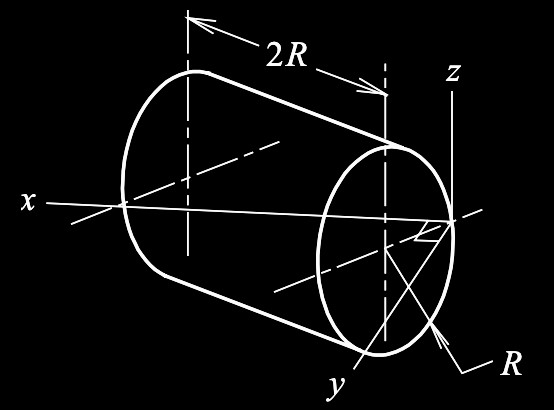
\includegraphics[scale=0.7,frame]{images/Q5_13.png}
% \end{figure}




\end{document}

